%!TEX root=../document.tex

\section{Architekturmöglichkeiten}
\subsection{Client-Server Architektur}
Bei der Client-Server Architektur, verbinden sich verschiedene Clients auf einen oder mehreren Servern, um Daten auszutauschen. Man hat dadurch zentrale Instanzen, welche für den Aufbau und Datenaustausch im Netzwerk essenziell sind.
Eine der wichtigsten Fragen bei der Client-Server Architektur ist, wie 'wieviel' am Client hinsichtlich der Tiers (View, Application,Data) liegt. Je weniger am Client liegt, desto schneller können auf Änderungen reagiert werden, da die Änderungen nur am Server vorgenommen werden müssen.
\begin{figure}[htbp] 
	\centering
	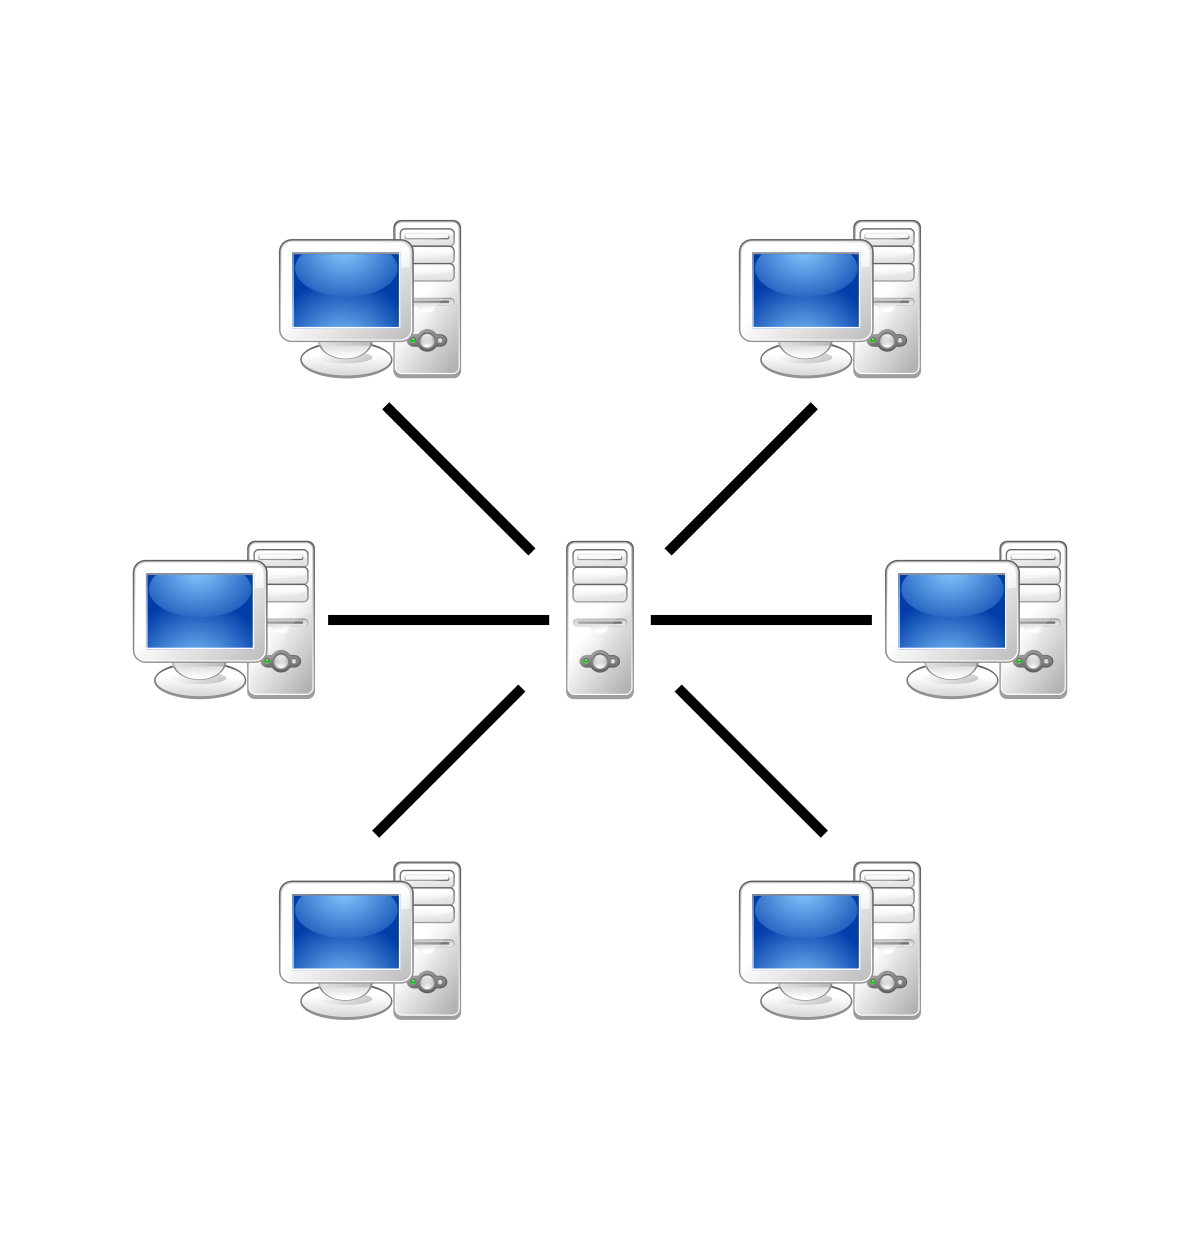
\includegraphics[width=0.5\textwidth]{images/client_server.PNG}
	\caption{Client-Server Architektur}
	\label{fig:Bild1}
\end{figure}

\subsubsection{Vorteile}
\begin{itemize}
	\item Performance (Rechenzeit, Speicherverbrauch) auf Server auslagern
	\item Plattformunabhängig (Business-Topic)
\end{itemize}

\subsubsection{Nachteile}
\begin{itemize}
	\item Single Point of Failure
	\item Erreichbarkeit (IP,Netzwerk-ID,Online)
	\item Welche Tiers am Client?
\end{itemize}
\subsection{Peer-to-Peer Architektur}
Bei einer Peer-to-Peer Architektur gibt es keine zentrale Instanz. Die Daten werden zwischen den einzelnen Clients ausgetauscht und jeder hält die Daten lokal auf seinem eigenen Rechner.

\begin{figure}[htbp] 
	\centering
	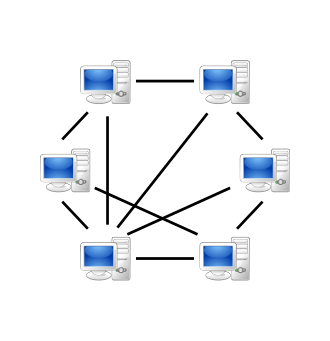
\includegraphics[width=0.7\textwidth]{images/p2p.PNG}
	\caption{Peer-to-Peer Architektur}
	\label{fig:Bild2}
\end{figure}

\subsubsection{Vorteile}
\begin{itemize}
	\item Skalierbarkeit erfolgt automatisch
	\item Verfügbarkeit
\end{itemize}
\subsubsection{Nachteile}
\begin{itemize}
	\item Interkommunikation (zentrale Authentifizierung fehlt)
	\item Deployment muss zentralisiert sein
	
\end{itemize}
\subsection{Gewählte Architektur}
Es wurde auf eine Client-Server Architektur gesetzt, da bei einer Client-Server ein zentraler Server zur Verfügung steht. Da sich alle Clients eine Einkaufsliste teilen, würde eine zentrale Datenbank Sinn ergeben.

Bei einer Peer-to-Peer Architektur würden Daten die nur lokal auf einem Client liegen. Hat dieser eine Änderung vorgenommen, wäre der Traffic, da dieser mit jedem Client kommunizieren muss anstatt mit einer zentralen Instanz, sehr hoch.
\section{Gewählte Datenbank - Firebase}
Firebase ist eine Real-Time Datenbank, die kostenlos von Google zur Verfügung gestellt wird. Firebase synchronisiert die Daten automatisch und unterstützt eine offline Synchronisation. Die Daten werden als JSON-Files abgespeichert. Firebase unterstützt Android und IOS Applikationen, sowie Webapplikationen.

Es werden APIs für alle gängigen Programmiersprachen angeboten.


\section{Alternativen}
\subsection{Couchbase Mobile}
Genau wie Firebase, bietet Couchbase Mobile eine Datenbank zur Verfügung, welche automatisch Daten zwischen den Clients synchronisiert. Couchbase speichert die Daten in JSON-Files ab. 

Hier werden ebenfalls APIs für die gängigen Programmiersprachen angeboten.

\subsection{RethinkDB}
Es werden Daten über JSON gespeichert. Es eignet sich für das Builden von skalierbaren mobilen Applikationen. Die Verbindung über das Web funktioniert sehr gut, da RethinkDB direkt über das HTTP's Request-Response gemapped wird.

RealthinkDB unterscheidet sich zu Firebase in 3 grundlegenden Punkten:
\begin{itemize}
	\item Die API ist Open-Source. Es kann ohne Restriktionen in der eigenen Infrastruktur deployed werden.
	\item Realtime Sync APIs sind auf das synchronisieren von Dokumenten beschränkt, während RethinkDB eine "general purpose Database" ist.
	\item RethinkDB wurde designed um direkt von einer Applikation-Server aufgerufen zu werden, anstatt vom Web
\end{itemize}

\section{Umsetzung}
Es wurde generell folgendes Tutorial umgesetzt \textbf{https://inducesmile.com/android/a-simple-android-todo-list-app-with-recyclerview-and-firebase-real-time-database/}. Es wird nicht auf das Tutorial generell eingegangen, sondern die Basics erklärt wie man Firebase grundlegend verwenden kann.

\subsection{Firebase einrichten}
Auf der Seite von Firebase ist es möglich ein neues Projekt einzurichten. Man kann nun ein google-services.json runterladen und dieses in das Android Projekt einfügen. Dieses JSON beinhaltet die Konfiguration der Firebase-Datenbank.

Im Gradle Build-File muss man google-services und Firebase als Dependency hinzufügen und dieses service anschließend applyen.

In den Einstellungen von Firebase wurde der Einfachkeit halber, die Datenbankrechte für das Lesen und Schreiben auf true gesetzt. Somit könnte sich jeder auf die Datenbank verbinden, der die Konfiguration der DB kennt.

In Java muss man um Daten zu pushen lediglich eine Instanz der DB erstellen und pushen:
\begin{lstlisting}
databaseReference = FirebaseDatabase.getInstance().getReference();

 databaseReference.push().setValue(taskObject);
\end{lstlisting}
\section{APK builden}